\chapter{Sprint 7 - Summary}

At the start of sprint 7, the team had Easter break from April 13 until the April 16. After Easter, the team acquired new high-speed servos and the variable pitch quadcopter was fully assembled. \\ 

After assembly the positioning of the servos were considered to be imprecise and new mounting brackets have been 3D-printed to ensure the same servo mount position for all servos.\\

For Qualisys, the room at KIC has been mapped, so that the quadcopter is automatically turned off as a safety feature when approaching the boundaries of the room. This reduces the chances of damage to the vehicle as well as the facility and people involved. \\

Concerning vibrations, the team is still experiencing problems. To investigate the source of the vibrations, vibrations have been recorded for several operating situations. Also, with and without dampening on the IMU. These data are plotted in Matlab and filters are applied to determine which filter is the best suited for our situation and noise. Additionally, an analog low pass filter and smoothing capacitor has been placed with the IMU.  

%% Vi hadde   95% scope completed og ikke noe scope change 
%% Var bare "Tune Radio Controller" som blø flyttet over til neste sprint

\section{Completion and Scope Change}

In sprint 7, 95\% of tasks were completed and there was no changes in scope. 


\begin{figure}[H]
    \centering
         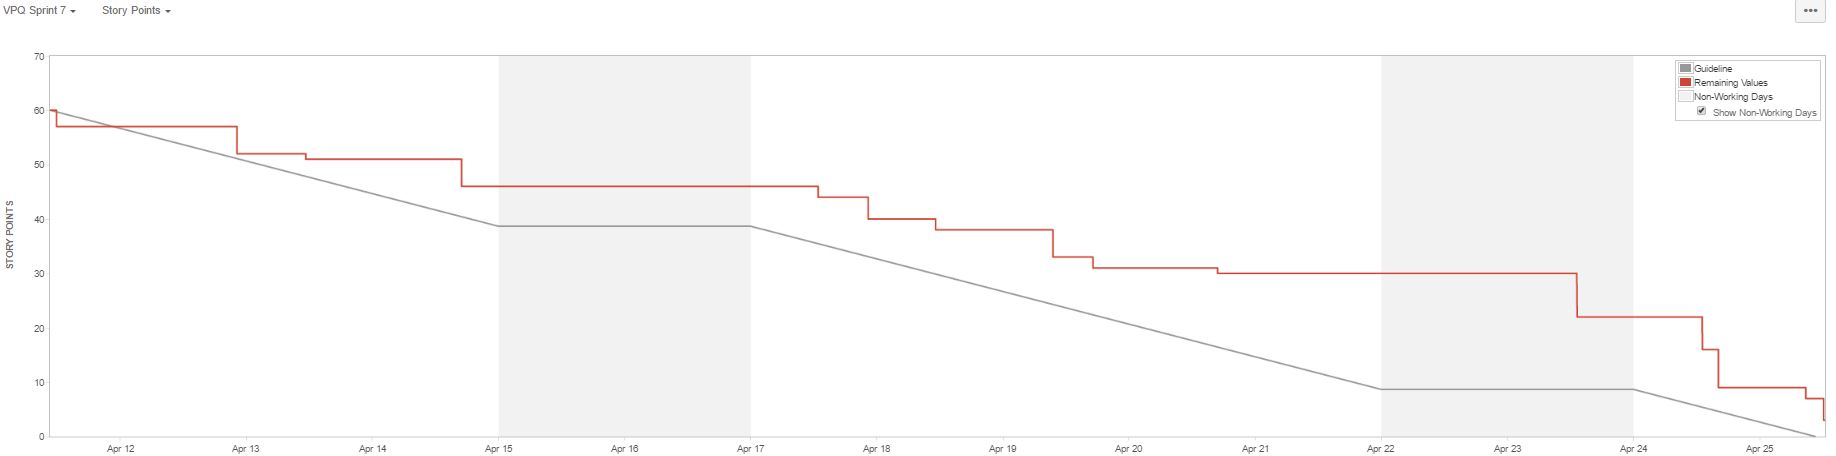
\includegraphics[width = 1\textwidth]{VAPIQ-PICTURES/BDSprint7}
      \caption{Burndown Chart Sprint 7}
    \label{fig:bds7}
\end{figure} 

\textbf{Project plan status, Sprint 7:}
\begin{itemize}
        \item Documentation ,\textbf{In progress}
        \item Tweak Flight Controller, VPQ ,\textbf{In Progress}
        \item Integrate Controller To Flight Controller ,\textbf{In progress}
        \item Testing And Comparison, \textbf{Postponed}
    \end{itemize}



